\documentclass{article}

\usepackage{lipsum}
\usepackage{amsfonts}
\usepackage{amsmath}
\usepackage{amsthm}
\usepackage{graphicx}
\usepackage{epstopdf}
\usepackage{algorithmic}
\ifpdf%
  \DeclareGraphicsExtensions{.eps,.pdf,.png,.jpg}
\else
  \DeclareGraphicsExtensions{.eps}
\fi
\usepackage{amsopn}
\DeclareMathOperator{\diag}{diag}
\usepackage{booktabs}
\usepackage{bbm}
\usepackage{bm}
\usepackage{caption}
\usepackage{subcaption}
\usepackage[utf8]{inputenc}
\usepackage[T1]{fontenc}
\usepackage[margin=1.5in]{geometry}
\usepackage{hyperref}

\newcommand{\norm}[1]{\left\lVert#1\right\rVert}
\newcommand{\normtwo}[1]{\left\lVert#1\right\rVert_2}
\newcommand{\abs}[1]{\left\lvert#1\right\rvert}
\newcommand{\mat}[1]{\bm{{#1}}}
\renewcommand{\vec}[1]{\bm{{#1}}}
\newcommand{\lequiv}{\Leftrightarrow}
\newcommand{\bigO}[1]{\mathcal{O}\!\left(#1\right)}
\newcommand{\ceil}[1]{\left\lceil #1 \right\rceil}
\newcommand{\floor}[1]{\left\lfloor #1 \right\rfloor}
\newcommand{\sfrac}[2]{#1/#2}
\newcommand{\hquad}{\enskip}
\newcommand{\expected}[1]{\mathbb{E}\left[#1\right]}
\newcommand{\mspan}[1]{\text{span}\left( #1 \right)}
\newcommand{\prob}[1]{P\left(#1\right)}
\newcommand{\probt}[1]{P\left( \text{#1} \right)}
\newcommand{\condprob}[2]{P\left(#1 \:|\: #2\right)}
\newcommand{\condprobt}[2]{P\left(\text{#1} \:|\: \text{#2}\right)}
\newcommand{\bayes}[2]{\frac{\condprob{#2}{#1}\prob{#1}}{\prob{#2}}}
\newcommand{\bayesx}[3]{\frac{\condprob{#2}{#1}\prob{#1}}{\condprob{#2}{#1}\prob{#1} + \condprob{#2}{#3}\prob{#3}}}
\newcommand{\sech}{\text{sech}}
\newcommand*{\vertbar}{\rule[-1ex]{0.5pt}{2.5ex}}
\newcommand*{\horzbar}{\rule[.5ex]{2.5ex}{0.5pt}}
\newcommand{\vect}[2]{\underline{{#1}}_{{#2}}}
\newcommand{\basisp}[1]{\underline{{p}}_{{#1}}}
\newcommand{\basisq}[1]{\underline{{q}}_{{#1}}}
\newcommand{\coeff}[1]{\underline{{a}}_{{#1}}}
\newcommand{\bestfit}{\underline{\bar{x}}}
\newcommand{\grad}{\nabla}
\newcommand{\laplace}{\Delta}
\newcommand{\setbar}{\:\middle|\:}
\renewcommand{\div}{\grad \cdot}
\renewcommand{\Re}{\text{Re}}

\begin{document}
\section{Learning Aggregation-Based Interpolation}

The edge-based convolution network we are using currently outputs a matrix that contains the same sparsity (or a subset of) the graph that it was given.  This means that it can be difficult to directly output some matrix with a different sparsity pattern without some intermediate transformation.

Denote $Agg$ the tentative aggregation operator without smoothing, for example,
\begin{equation}
Agg =
\begin{bmatrix}
  1 & \\
  1 & \\
  1 & \\
  & 1 \\
  & 1
\end{bmatrix},
\end{equation}
would correspond to a $5 \times 5$ system with two aggregates, the first containing nodes $1-3$ and the second containing nodes $4$ and $5$.  Let $\mat{A}$ be the system being solved and $\mat{P}$ the interpolation operator, i.e. that obtained by running some relaxation scheme on $Agg$.

One way to solve this is to first form $\mat{\hat{P}}$ as usual using the graphnet's node and edge convolutions.  This will give us a matrix that has the same sparsity pattern as $\mat{A}$.  Continuing the example from above, we may obtain some $\mat{\hat{P}}$ like
\begin{equation}
\mat{\hat{P}} =
\left[\begin{array}{@{}ccc|cc@{}}
  \sfrac{1}{2} & \sfrac{1}{3} & & & \\
  \sfrac{1}{2} & \sfrac{1}{3} & \sfrac{1}{3} & & \\
               & \sfrac{1}{3} & \sfrac{1}{3} & \sfrac{1}{3} &\\
               &              & \sfrac{1}{3} & \sfrac{1}{3} & \sfrac{1}{2} \\
  &              &              & \sfrac{1}{3} & \sfrac{1}{2}
\end{array}\right],
\end{equation}
with nodes to the left of the bar signifying those belonging to the first aggregate, and those to the right belonging to the second aggregate.

Then, we form $\hat{Agg}$, which is the $Agg$ operator from above except with its columns normalized in the $1$-norm.  This would give
\begin{equation}
\hat{Agg} =
\begin{bmatrix}
  \sfrac{1}{3} & \\
  \sfrac{1}{3} & \\
  \sfrac{1}{3} & \\
  & \sfrac{1}{2} \\
  & \sfrac{1}{2}
\end{bmatrix}.
\end{equation}
Now, we can ``collapse'' the columns of the nodes corresponding to each aggregate by averaging them together.  This can be written concretely as
\begin{equation}
\mat{P} = \mat{\hat{P}}\hat{Agg} = \begin{bmatrix}
  0.277 & \\
  0.333 & \\
  0.222 & 0.166 \\
  0.111 & 0.416 \\
  & 0.416 \\
\end{bmatrix},
\end{equation}
which gives a reasonable sparsity pattern for the interpolation, given $Agg$.  Note that if we view this as a graph, we get edge connections between aggregates ``for free'', which is exactly what is wanted.

\section{Problem Setup}
The specific problem being solved is a diffusion problem with Neumann boundary conditions.  To test the feasibility of the method, results were fixed for one problem and the networks/methods allowed to ``overfit'' to see if some reasonable solution is obtained.  Aggregates were generated with Lloyd aggregation, using a seed ratio of $0.25$.  This gives a relatively high number of small aggregates, which may be somewhat unwanted in practice.

\begin{figure}[h]
  \includegraphics[width=\textwidth]{figures/diffusion-lloyd-aggregates.pdf}
  \caption{Specific problem being solved, with aggregate information.}
  \label{fig:lloyd_aggregates}
\end{figure}

\section{Numerical Results}
Using Lloyd to generate the aggregates and then generating $\mat{P}$ with a Jacobi prolongation smoother results in an AMG method with a convergence factor of approx. $0.6874$, as measured by the loss function.  This will be used as a baseline to compare the following results.

All of the following plots are using the same random seeds, meaning both Lloyd aggregates and test vectors for the AMG loss should remain fixed for each training iteration.

\begin{figure}[h]
  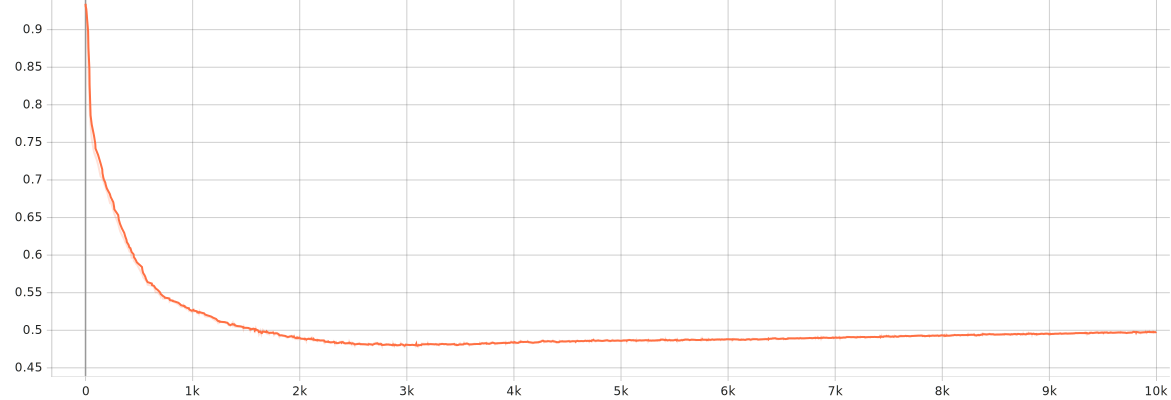
\includegraphics[width=\textwidth]{figures/learn_p_directly.pdf}
  \caption{Loss function when directly optimizing the nonzero entries of $\mat{P}$.  Using Adam optimizer with a learning rate of $0.01$.}
  \label{fig:loss_p}
\end{figure}

\begin{figure}[h]
  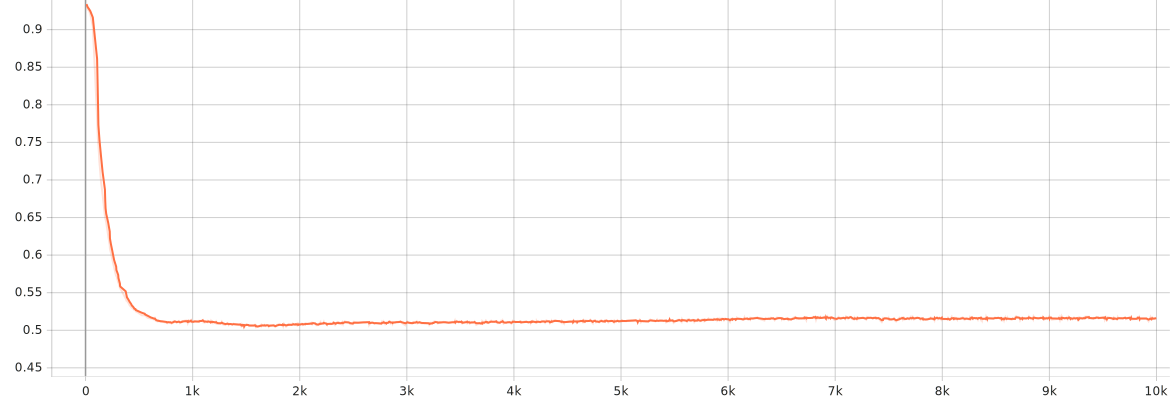
\includegraphics[width=\textwidth]{figures/learn_p_hat.pdf}
  \caption{Loss function when optimizing the nonzero entries of $\mat{\hat{P}}$, then forming $\mat{P}=\mat{\hat{P}}\hat{Agg}$.  Using Adam optimizer with a learning rate of $0.01$.}
  \label{fig:loss_p_hat}
\end{figure}

\begin{figure}[h]
  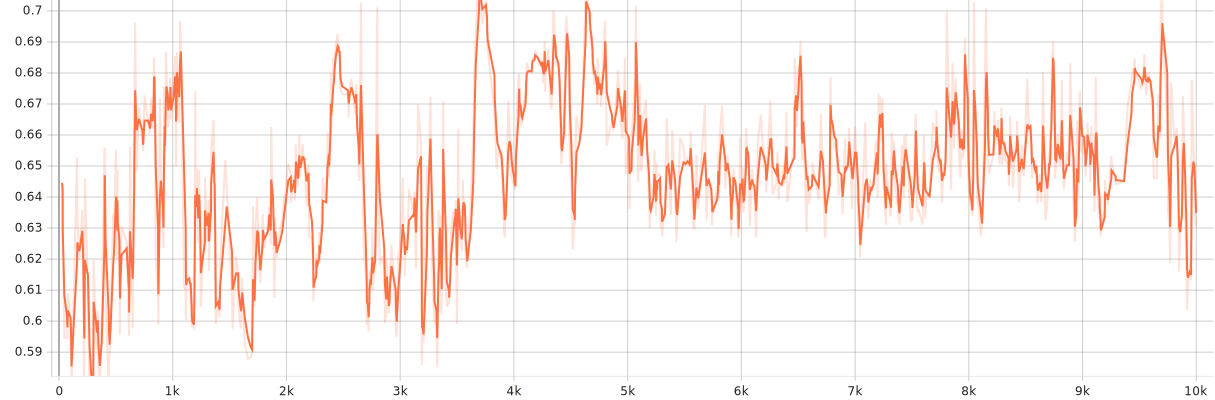
\includegraphics[width=\textwidth]{figures/learn_graphnet.pdf}
  \caption{Loss function when using a Graphnet to generate $\mat{\hat{P}}$.  Using Adam optimizer with a learning rate of $10^{-5}$.}
  \label{fig:loss_graphnet}
\end{figure}

\end{document}
